\section{创建 Account 继承层次}
\hfill\ctli{实验时间}{~2015~年~1~月~14~日}
\subsection*{【实验目的】}
\begin{enumerate}[topsep=0pt,partopsep=0pt,itemsep=0pt,parsep=0pt,label={\arabic*、}]
\item 掌握继承的概念。
\item 掌握不同继承方式的继承特性。
\end{enumerate}
\subsection*{【实验环境】}
\MyEnvironment
\subsection*{【实验内容】}
P522:12.10
\subsection*{【详细分析】}
创建一个银行账户的继承层次,表示银行的所有客户账户。所有的客户都能在他们的银行账户存钱、取钱,但是账户也可以分成更具体的类型。例如,一方面存款账户 SavingsAccount 依靠存款生利;另一方面,支票账户 CheckingAccount 对每笔交易(即存款或取款)收取费用。

创建一个类层次,以 Account 作为基类,SavingsAccount 和 CheckingAccount 作为派生类。基类 Account 应该包括一个 double 类型的数据成员 balance,表示账户的余额。该类应提供一个构造函数,接受一个初始余额值并用它初始化数据成员 balance。而且构造函数确认初始金额的有效性,保证它大于等于 0。如果小于 0,则需将其置为 0,并显示出错信息,表明该初始化余额是一个无效的值。该类应该提供三个成员函数:成员函数 credit 可以向当前余额加钱;成员函数 debit 负责从账户中取钱,并且保证账户不会透支。如果提取金额大于账户余额,函数将保持 balance 不变,并打印信息“取钱金额超过账户余额”;成员函数 getBalance 则返回当前 balance 的值。

派生类 SavingsAccount 不仅继承了基类 Account 的功能,而且还应提供一个附加的 double 类型数据成员 interestrate 表示这个账户的利率(百分比)。SavingsAccount 的构造函数应接受初始余额值和初始利率值,还应提供一个 pubilc 成员函数 calculateInterest,返回代表账户的利息的一个 double 值,这个值是 balance 和 interestrate 的乘积。注意:类 SavingsAccount 应继承成员函数 credit 和 debit,不需要重新定义。

派生类 CheckingAccount 不仅继承了基类 Account 的功能,还应提供一个附加的 double 类型数据成员 feechargepertransaction 表示每笔交易的费用。CheckingAccount 的构造函数应接受初始金额值和交易费用值。类 CheckingAccount 需要重新定义成员函数 credit 和 debit,当每笔交易完成时,从 balance 中减去 feechargepertransaction。重新定义这些函数时应用到基类 Account 的这两个函数来执行账户余额的更新。CheckingAccount 的 debit 函数只有当钱被成功提取时才应收取交易费。提示:定义 Account 的 debit 函数使它返回一个 bool 类型值,表示钱是否被成功提取。然后利用该值决定是否需要扣除交易费。

当这个层次中的类定义完毕后,编写一个程序,要求创建每个类的对象并测试它们的成员函数。将利息加到 SavingsAccount 对象的方法是:先调用它的成员函数 calculateInterest,然后将返回的利息传递给该对象的 credit 值。

(以上手敲)
\subsection*{【实验源码】}
{\linespread{1}
\lstinputlisting[caption={\tt Account.h}]{exp06/Account.h}
\lstinputlisting[caption={\tt Account.cpp}]{exp06/Account.cpp}
\lstinputlisting[caption={\tt SavingsAccount.h}]{exp06/SavingsAccount.h}
\lstinputlisting[caption={\tt SavingsAccount.cpp}]{exp06/SavingsAccount.cpp}
\lstinputlisting[caption={\tt CheckingAccount.h}]{exp06/CheckingAccount.h}
\lstinputlisting[caption={\tt CheckingAccount.cpp}]{exp06/CheckingAccount.cpp}
\lstinputlisting[caption={\tt exp01.cpp}]{exp06/exp01.cpp}
}
\subsection*{【实验结果】}
\begin{figure}[htp]
\centering
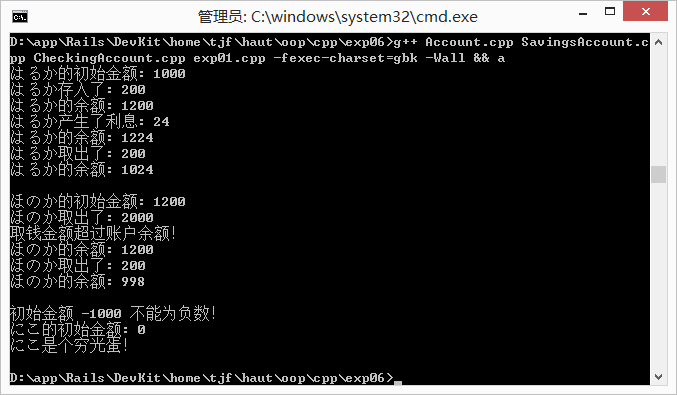
\includegraphics[width=\textwidth]{exp06/exp01.png}
\caption{\label{out06_01}Account 继承层次}
\end{figure}
\subsection*{【实验体会】}
这是一个掌握 C++ 继承的练习题。一个要注意的地方,和其他面向对象语言不同的是,C++ 在父类需要用 virtual 关键字来声明有可能在子类中重载的方法(并且声称这是为了性能)。子类的构造函数中可以调用父类的构造函数,子类的方法也可以调用父类的同名方法。这些特性减少了代码量,避免了代码冗余的产生。这个例子也很好地巩固了继承的概念。
